% !TeX encoding = utf-8
% !TeX program = pdflatex
% -*- coding:utf-8 mod:LaTeX -*-

% Paper 3 — IEEE Signal Processing Letters (SPL) version.
% v3 (2026-09-30): revised against the second pre-submission review
% (paper3/review2.md). Changes vs v2: conditional proposition for the
% generality claim; Table I made internally consistent (concatenated
% point estimates paired with concatenated bootstrap CIs) + Delta-AUROC
% with permutation tests; bin-wise label-permutation null for the
% post-hoc oracle (selection-optimism calibration); kk/ku/uu protocol
% decomposition incl. same-mixture K-vs-U comparison; multiple
% independent test seeds; SIR-controlled attribution sweep; title and
% keywords aligned with the mechanism (label-score misalignment, not
% "data leakage"); "at chance" softened to "no reliable positive
% discrimination"; 0-dB boundary provenance stated; FPR95 defined;
% abstract tightened; figures annotated (chance line, sigma notation).
% Page budget: SPL allows 4 pages + a 5th page of references only.

\documentclass[journal,letterpaper]{IEEEtran}
% IEEEtran.cls sets \ttdefault to pcr (Courier), whose TFM metrics are
% missing from BasicTeX; revert to cmtt so \texttt builds without error.
\renewcommand{\ttdefault}{cmtt}

\usepackage{graphicx}
\usepackage{booktabs}
\usepackage{amsmath,amssymb}
\usepackage{url}
\usepackage{xcolor}
\usepackage[mode=text]{siunitx}
\sisetup{locale=US}
\usepackage{hyperref}
\hypersetup{hidelinks, colorlinks=true, allcolors=black,
  pdfstartview=Fit, breaklinks=true}

\newcommand{\snr}{\mathrm{SNR}}

\begin{document}

\title{A Label--Score Alignment Pitfall in SNR-Conditioned OOD
Detection for Single-Channel Blind Source Separation}

\author{Bin~Nong, Weihong~Fu, and Zhuoyun~Jiang%
\thanks{Manuscript prepared 2026. B.~Nong is with Tianfu College of
Southwestern University of Finance and Economics, Mianyang 621000, China
(e-mail: nongbin@tfswufe.edu.cn). W.~Fu is with the School of
Telecommunications Engineering, Xidian University, Xi'an 710071, China.
Z.~Jiang is with the School of Health Science and Engineering,
University of Shanghai for Science and Technology, Shanghai 200093,
China.}%
\thanks{Digital object identifier: TODO (assigned by the journal).}%
\thanks{The authors used a generative AI assistant for coding support
and language polishing.}}

\markboth{IEEE Signal Processing Letters, 2026}%
{Nong \MakeLowercase{\textit{et al.}}: A Label--Score Alignment
Pitfall in SNR-Conditioned OOD Detection for SC-BSS}

\maketitle

\begin{abstract}
Evaluating out-of-distribution (OOD) detection for communication
signals is routinely conditioned on the operating SNR\@. We show this
conditioning is fragile to label misalignment. Storing per-source SNR
labels interleaved (\texttt{np.repeat}) while the scores they annotate
are stacked slot-wise (\texttt{np.tile}) manufactures a spurious
phenomenon in which two OOD scorer families appear complementary
across SNR and a training-free SNR-routed ensemble appears to lift
AUROC from $0.50$ to $0.625 \pm 0.031$. We formalize the failure as an
indexing-permutation confound and prove that whenever OOD scores drift
with SNR, \emph{any} label permutation that alters the per-bin SNR
composition converts that drift into spurious per-SNR separability
(routed weighted AUROC up to $0.746$). The same pipeline is then shown
to hide a second, independent misalignment---per-source labels swapped
alongside permutation-invariant alignment---with the opposite effect:
a genuine same-mixture detection margin (AUROC $0.54$) attenuated to
an apparent null. Randomness-oriented safeguards (multi-seed averaging,
significance tests, robustness batteries) detect neither error.
Doubly corrected, no post-hoc
scorer gives deployable \emph{pooled} discrimination (routed
$0.508 \pm 0.026$; five seeds, four independent test realizations);
a modest \emph{same-mixture} embedding margin
survives (prototype AUROC $0.54$, $0.60$--$0.65$ at SNR
${\geq}\,$\SI{5}{dB}), logit
scorers are inverted, and the margin collapses when the unknown source
is the weak one.
\end{abstract}

\begin{IEEEkeywords}
Blind source separation, open-set recognition, out-of-distribution
detection, evaluation methodology, label misalignment.
\end{IEEEkeywords}

\section{Introduction}
\label{sec:intro}

\IEEEPARstart{S}{ingle-channel} blind source separation (SC-BSS) of
co-frequency communication signals is increasingly paired with
per-source modulation identification~\cite{hou2022single,guo2024single},
and a deployed receiver must additionally \emph{reject} sources whose
modulation it has never seen---an open-set recognition
problem~\cite{scheirer2013open,li2023expert} for which post-hoc OOD
scorers of learned embeddings and logits
\cite{hendrycks2017msp,liang2018odin,liu2020energy,lee2018mahalanobis,du2022vos}
are the standard toolkit. Because OOD score distributions drift with
noise, communication-signal evaluation is routinely conditioned on the
operating SNR---per-SNR-bin profiles and weighted
averages~\cite{proakis2008digital,oshea2017intro,li2023expert}.

This letter shows that the conditioning step itself is a single point
of failure. A one-line labeling-convention mismatch misaligns every
known-pool score with the wrong SNR bin, and each ``per-SNR bin'' then
compares known and unknown pools at \emph{different} true SNRs: the
bins measure SNR separability, not OOD separability. The artifact is insidious precisely because it is
\emph{systematic}: multi-seed averaging, significance testing, and
robustness batteries are randomness-oriented safeguards, and they
cannot detect deterministic pipeline errors
\cite{kapoor2023leakage,musgrave2020reality}. We contribute:
(i)~a formalization of the failure as an indexing-permutation confound,
including a proposition giving the exact conditions (SNR-dependent
scores plus a composition-changing label permutation) under which
\emph{any} such misalignment manufactures spurious per-SNR gains
(routed weighted AUROC up to $0.746$), and why the trusted checks fail
to catch it;
(ii)~a deployment-faithful evaluation protocol (verified alignment,
strict train/reference/test separation, unknown-free calibration,
operating-point metrics, protocol-wise and same-mixture comparisons,
independent test realizations)---whose same-mixture control exposes a
\emph{second}, independent label misalignment in the same pipeline
(per-source labels swapped alongside permutation-invariant alignment),
with the opposite sign: it attenuates a genuine margin to an apparent
null; and (iii)~the doubly corrected study on an open-set SC-BSS
benchmark (six scorers, five seeds, two backbones, four independent
test sets, LOMO splits, per-class near/far-OOD breakdowns, a calibrated
operating point, a controlled interference sweep): no deployable
\emph{pooled} discrimination, but a modest \emph{same-mixture}
embedding margin that is inverted for logit scorers and collapses when
the unknown source is weak.

\section{Open-Set SC-BSS Setup}
\label{sec:setup}

\emph{Signal model and SNR definition.} We study the two-source
co-frequency mixture $y(t) = \alpha_1 s_1(t) + \alpha_2 s_2(t) + n(t)$
at complex baseband. Each $s_i$ is a unit-power synthetic waveform
(\SI{16}{kHz} sampling, 256 symbols at 16 samples/symbol,
root-raised-cosine pulse shaping with roll-off 0.35, 3-tap complex
Gaussian multipath normalized to unit gain, carriers
\SI{2000}{Hz}/\SI{2005}{Hz} with $\pm$\SI{5}{Hz} uniform jitter,
$T = 4096$ samples~\cite{proakis2008digital}), mixed with
$\alpha_1 = \alpha$, $\alpha_2 = 1 - \alpha$, $\alpha \sim U(0.4,
0.6)$, plus AWGN\@. Throughout, SNR denotes the \emph{mixture} SNR
$\snr_{\text{mix}} = 10\log_{10}\bigl(\mathbb{E}|\alpha_1 s_1 +
\alpha_2 s_2|^2 / \mathbb{E}|n|^2\bigr)$. Since the sources are
unit-power, the per-source SNR of source $i$ is
$\snr_i = \snr_{\text{mix}} + 10\log_{10}\!\bigl(\alpha_i^2 /
(\alpha_1^2 + \alpha_2^2)\bigr) \approx \snr_{\text{mix}} -
\SI{3}{dB}$ under near-equal mixing, and the SIR
$20\log_{10}(\alpha_1/\alpha_2)$ sweeps $[-3.5, 3.5]$ dB with the
$\alpha$ draw. The per-source label stored by the evaluation pipeline
is this shared $\snr_{\text{mix}}$.

\emph{Modulations, protocols, pools.} Modulations split into known
$\mathcal{K} = \{$BPSK, QPSK, 8PSK, 16QAM$\}$ (training only) and
held-out $\mathcal{U} = \{$64QAM, $\pi$/4-DQPSK, MSK, OFDM-QPSK$\}$;
test protocols are kk/ku/uu by the number of unknown sources
(deterministic seed 99999; 192 kk, 192 ku, and 96 uu mixtures per bin
of the grid $\{-10, -5, \dots, 20\}$ dB). The \emph{known pool} holds
both slots of the kk mixtures and the \emph{unknown pool} the OOD slot
of each ku mixture plus both slots of uu (2688 sources each; 384 per
SNR bin). The separator is a lightweight complex-valued CNN with
complex squeeze-and-excitation (C-SE) attention ($\sim$69K parameters)
plus a shared per-source modulation head (64-d embedding $z$, 4 logits
$f$), trained with permutation-invariant SI-SDR + cross-entropy
\cite{kolbaek2017pit,leroux2019sdr} on known modulations only.
Closed-set reference points (kk): SI-SDR $-0.89$ dB pooled;
truth-anchored modulation accuracy $0.52$---an interference-limited
regime (SIR~$\approx 0$~dB), the stress test under which per-source
OOD detection would have to operate.

\emph{Scorers and leakage control.} Six post-hoc OOD scorers (larger =
more OOD) are applied per source: Energy $-\log\sum_k
e^{f_k}$~\cite{liu2020energy}, MSP~\cite{hendrycks2017msp},
ODIN~\cite{liang2018odin}, Mahalanobis~\cite{lee2018mahalanobis},
nearest-prototype distance, and a VOS-inspired (training-free,
post-hoc) virtual-outlier distance~\cite{du2022vos}, all at literature
defaults fixed \emph{a priori} (ODIN $T{=}1000$,
$\varepsilon{=}0.005$; Mahalanobis shared covariance, shrinkage 0.1;
VOS-inspired scale 2, 100 outliers/class); every fitted quantity (prototypes, covariance,
virtual outliers, thresholds) is estimated on a disjoint reference
pool (seed 88888, kk protocol), and \textbf{no unknown-class sample is
used for any fitting, selection, or calibration step}---the routing
boundary (\SI{0}{dB}) is a development-time choice, fixed from the
validation-profile crossover of the original study and frozen before
any corrected-test evaluation, and the LOMO study selects
boundaries exclusively on a further pseudo-OOD validation split (seed
77777). The rejection threshold $\tau$ is the 95th percentile of
known-pool reference scores (5\% false-rejection target). The a-priori
\emph{SNR-routed} score uses Energy at $\snr \leq \SI{0}{dB}$ and
Prototype otherwise.

\begin{figure*}[!t]
\centering
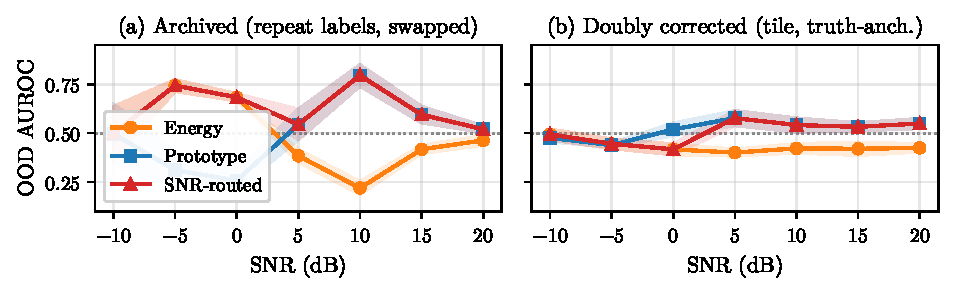
\includegraphics[width=0.67\textwidth]{figures/fig_artifact_vs_corrected.pdf}
\caption{Per-SNR OOD AUROC (5-seed mean $\pm$ std) under (a) the
archived pipeline (repeat SNR labels, swapped pool membership) and
(b) the doubly corrected evaluation (tile labels, truth-anchored). The
apparent complementarity---Energy peaking at low SNR, Prototype at high
SNR---is manufactured by the label misalignments; corrected, the routed
profile is flat near chance (dotted line).}
\label{fig:money}
\end{figure*}

\begin{figure}[!t]
\centering
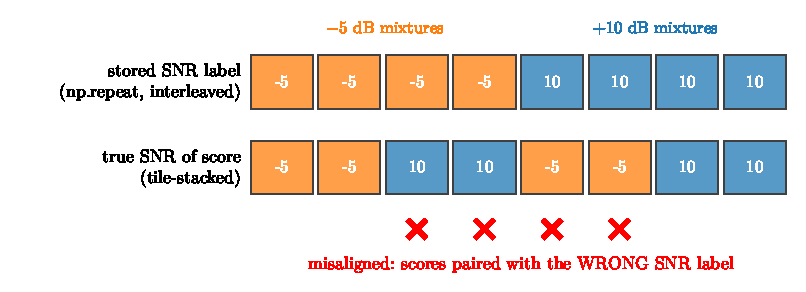
\includegraphics[width=\columnwidth]{figures/fig_pitfall_mechanism.pdf}
\caption{The misalignment. Scores are stacked tile-wise (all slot-1
entries, then all slot-2), so their true SNR sequence alternates blocks;
the stored labels repeat each mixture's SNR interleaved. Entries past
the slot boundary (red crosses) are paired with the wrong SNR (up to
\SI{15}{dB})---an indexing-permutation mismatch $\sigma_q(j) \neq
\sigma_\ell(j)$ (Sec.~\ref{sec:pitfall}).}
\label{fig:mechanism}
\end{figure}

\section{The Pitfall}
\label{sec:pitfall}

\emph{Mechanism and formalization.} Index the test mixtures
$m = 1, \dots, N$ in SNR-block order. The evaluation stores per-source
scores $q_j$ stacked \emph{tile-wise} and per-source SNR labels
$\ell_j$ written \emph{interleaved} (\texttt{np.repeat}), so score $j$
belongs to mixture $\sigma_q(j) = ((j-1) \bmod N) + 1$ but is paired
with the label of mixture $\sigma_\ell(j) = \lceil j/2 \rceil$: an
indexing-permutation mismatch $\sigma_q \neq \sigma_\ell$
(Fig.~\ref{fig:mechanism}). Binning by $\ell$ assigns to stored bin
$b$ known scores whose \emph{true} SNRs differ from $b$ wherever the
permutations disagree; the exactly labeled unknown pool is unaffected,
so each per-bin AUROC measures the score's \emph{SNR separability},
not OOD separability, with a magnitude set by the deterministic
label--truth SNR gap (up to \SI{15}{dB} here). A one-line audit
exposes the corruption: binning the
known pool's stored \emph{modulation} labels by the stored SNR labels
gives impossible per-bin class counts ($114/96/100/74$; the protocol
contributes exactly $96$ mixtures per known modulation per true bin);
the corrected (tile) labels recover $96/96/96/96$.

\emph{A conditional proposition.} The artifact instantiates a general
confound whose conditions can be stated exactly.

\textbf{Proposition 1.} \emph{Let $S$ be an OOD score that is
conditioned on the true SNR $C$ but carries no OOD information beyond
it, $S \perp O \mid C$ for the OOD label $O \in \{k, u\}$, and whose
family $\{p(s \mid c)\}$ is stochastically ordered in $c$. If the
stored labels assign to bin $b$ a known pool whose true-SNR
distribution $P(C_k \mid \ell_k {=} b)$ has mass at $c \neq b$, while
the exactly labeled unknown pool sits at $b$, then the per-bin AUROC
$A_b = P(S_u {>} S_k \mid \ell_u {=} \ell_k {=} b) \neq \tfrac{1}{2}$,
with sign set by $b - \mathbb{E}[C_k \mid \ell_k {=} b]$.}

\emph{Sketch.} Marginalizing the corrupted known labels,
$A_b = \int P(S_u {>} S_k \mid c_u {=} b, c_k)\, dP(c_k \mid
\ell_k {=} b)$; under $S \perp O \mid C$ the integrand equals
$\tfrac{1}{2}$ at $c_k = b$ and moves monotonically with $b - c_k$ by
stochastic ordering, so any mass away from $b$ biases $A_b$.
\hfill$\square$

The conditions are exact: the score must drift with SNR (all six
scorers here do) and the permutation must change the per-bin SNR
composition (block-aligned shifts are exact no-ops, below).

\emph{Generality: permutation study.} The repeat-vs-tile bug is one
member of the class delimited by Proposition~1. Re-binning
the \emph{corrected} scores with synthetic label permutations $\pi$
over the known pool (5-seed mean weighted AUROC of the a-priori routed
score): $\pi_{\text{identity}} = 0.508$; $\pi_{\text{repeat}}$ (the
original bug, isolated on clean pools) $= 0.619$;
$\pi_{\text{reverse}} = 0.746$; ten uniform
\emph{random} permutations $= 0.632 \pm 0.005$; block-structure
preserving shifts are exact no-ops ($0.508$). Per-bin AUROCs reach
$0.85$ under $\pi_{\text{reverse}}$. Two confounds combine: mismatched
known bins separate by their true-SNR composition (under
$\pi_{\text{random}}$ each bin approximates ``full known pool vs
unknown at $b$'', exposing opposite monotone SNR gradients for Energy
and Prototype), and the fixed a-priori routing rule harvests both
gradients by construction. Notably,
single-scorer weighted averages stay near $0.48$--$0.51$ under every
$\pi$: the average can look innocent while the per-bin structure is
entirely spurious---which is exactly how the artifact presented as
\emph{complementarity} rather than as a global lift. Label--index
alignment is therefore not an implementation detail but a
confound-control condition for conditioned evaluation.

\emph{The manufactured phenomenon.} Under the buggy labels the
benchmark presented a perfect complementarity (Prototype $0.84$ AUROC
at \SI{10}{dB}, collapsing below \SI{0}{dB}; Energy $0.74$ at
\SI{-5}{dB}), and routing on it
appeared to lift the pair-weighted AUROC from $0.50$ to $0.625 \pm
0.031$ (five seeds) against a post-hoc oracle of $0.681$
(Fig.~\ref{fig:money}a). It also produced a full supporting narrative:
``graceful degradation'' under simulated SNR-estimation error,
``robustness'' to SIR/timing/carrier perturbations, ``consistent''
ablations.

\emph{Why it survives the standard checks.} The misalignment is a
deterministic function of the data layout, identical for every seed
and condition: multi-seed averaging \emph{confirms} it ($\pm 0.031$),
and significance tests are significant precisely because the
SNR-mismatch signal is real---what is wrong is the bins'
interpretation. Robustness perturbations act on the signals, not the
label geometry, so each pass reads as independent evidence; and the
pattern is mechanistically narratable (``confidence inverts at high
SNR''), which is how it survives internal scrutiny. The critical check
is label--score alignment against regenerated data, which standard
seed- and robustness-based validation does not capture.

\emph{How it was caught.} Replacing the oracle SNR in the router with
a real blind SNR estimator (median-eigenvalue subspace estimator,
\SI{0.51}{dB} overall RMSE; classical M2M4 is inadequate
here~\cite{pauluzzi2000snr}) required pairing waveform-derived
estimates with stored scores; the alignment verification written for
that purpose failed immediately and exposed the repeat-vs-tile
mismatch.

\section{Corrected Protocol and Results}
\label{sec:corrected}

\emph{Protocol.} (i) \textbf{Verified label alignment}: every dumped
label array is checked against regenerated data (sequence equality,
per-bin counts, per-bin label multisets). (ii) \textbf{Strict
separation}: training, the reference pool (seed 88888), and the test
set (seed 99999) never mix; all fitted OOD quantities come from the
reference pool. (iii) \textbf{Unknown-free calibration}: $\tau$ is the
95th percentile of known-pool reference scores; no unknown-class data
is used for any fitted quantity, and the routing boundary is frozen
from development (Sec.~\ref{sec:setup}). (iv) \textbf{Operating-point metrics}---Det@$\tau$, FPR95
(known-pool rejection rate at 95\% unknown detection),
OSCR~\cite{dhamija2018oscr}, joint known/unknown
accuracy---alongside per-SNR and pooled AUROC\@. (v)~\textbf{Protocol
decomposition}: pooled AUROC could confound modulation novelty with
mixture composition (the known pool draws only from kk mixtures); we
report protocol-wise AUROCs and a \emph{same-mixture} comparison
(known vs unknown slot within each ku mixture), which removes the
confound by construction (uu mixtures contain no known source and
contribute no such control). (vi)~\textbf{Independent test
realizations}: beyond the deterministic test seed 99999, the full
protocol is repeated on three further independent test sets (seeds
100001--100003). Seed standard deviations describe training-run
variability; bootstrap CIs describe test-sample variability.

\begin{table}[!t]
\centering
\caption{Weighted-average per-SNR AUROC, artifact vs corrected labels
(5 seeds, mean $\pm$ seed std); corrected pooled AUROC on the
concatenated 5-seed samples ($13440$ + $13440$) with its own 95\%
bootstrap CI; $\Delta = \text{AUROC} - 0.5$; $p$ from a two-sided
label-permutation test ($B = 10^4$). Corrected columns are doubly
corrected (tile SNR labels, truth-anchored membership and reference
fit); the artifact column reproduces the archived mislabeled dumps.
The oracle's margin over routed ($0.042$) splits into per-bin
max-selection optimism (null $0.518$ [$0.513, 0.523$]) plus the small
genuine embedding margin ($p = 5{\times}10^{-4}$ vs the null).}
\label{tab:master}
\scriptsize\setlength{\tabcolsep}{3pt}
\begin{tabular}{lccc}
\toprule
Scorer & Artifact wavg & Corrected wavg & Corrected pooled [95\% CI], $\Delta$ ($p$) \\
\midrule
Energy        & $0.487\pm0.032$ & $0.431\pm0.023$ & $0.450$ [$0.443, 0.456$], $-0.050$ ($10^{-4}$) \\
MSP           & $0.435\pm0.012$ & $0.394\pm0.007$ & $0.405$ [$0.398, 0.411$], $-0.095$ ($10^{-4}$) \\
ODIN          & $0.495\pm0.030$ & $0.435\pm0.021$ & $0.460$ [$0.453, 0.466$], $-0.040$ ($10^{-4}$) \\
Mahalanobis   & $0.526\pm0.043$ & $0.529\pm0.056$ & $0.525$ [$0.517, 0.531$], $+0.025$ ($10^{-4}$) \\
Prototype     & $0.502\pm0.008$ & $0.518\pm0.022$ & $0.509$ [$0.502, 0.516$], $+0.009$ ($0.008$) \\
VOS-inspired  & $0.502\pm0.008$ & $0.518\pm0.022$ & $0.509$ [$0.502, 0.516$], $+0.009$ ($0.01$) \\
\midrule
SNR-routed    & $0.625\pm0.031$ & $0.508\pm0.026$ & --- \\
Oracle (6, post-hoc) & $0.681\pm0.039$ & $0.550\pm0.041$ & --- \\
\bottomrule
\end{tabular}
\end{table}

\emph{A second misalignment, exposed by the same-mixture control.}
The same-mixture comparison required by protocol item (v) contradicted
the pooled corrected numbers; the audit traced it to a second label
misalignment in the dump stage of the
original pipeline: permutation-invariant (PIT) alignment anchored the
waveforms, embeddings, and logits to the true sources but swapped the
per-source \emph{labels} (modulation indices and OOD flags) with the
output slots. At SIR~$\approx 0$~dB the swap rate is $\approx 0.50$,
so the ku-derived pools were about half contaminated and every
ku-dependent AUROC was attenuated toward chance (closed-set accuracy
recovers from $0.42$ to $0.52$ when truth-anchored); the kk/uu pools,
the reference pool, and the SNR labels are unaffected, as is
Sec.~\ref{sec:pitfall}'s analysis in kind. The failure class is
Proposition~1's---deterministic label misalignment---with the opposite
sign: it \emph{erases} structure. \textbf{All corrected
numbers below are truth-anchored.}

\emph{Corrected results.} Under verified, truth-anchored labels no
scorer provides practically useful \emph{pooled} discrimination
(Fig.~\ref{fig:money}b; Table~\ref{tab:master}): the routed ensemble
reaches $0.508 \pm 0.026$ and stays flat across three further
independent test realizations (seeds 100001--100003, routed
$0.501$--$0.517$). The deviations from chance are structured:
the logit scorers sit \emph{below} chance (MSP $\Delta = -0.095$;
Energy $\Delta = -0.050$; permutation $p = 10^{-4}$)---the known-class
head is confidently wrong on unknown modulations---while the embedding
scorers sit marginally above (Mahalanobis $\Delta = +0.025$;
Prototype/VOS $\Delta = +0.009$), driven by far-OOD classes and
high-SNR bins (below). The post-hoc oracle ($0.550$) exceeds its
correlation-preserving permutation null ($0.518$,
$p = 5{\times}10^{-4}$)---a bound, not a deployable score
(Table~\ref{tab:master}). Under truth-anchored labels the intervention
battery leaves the routed score near chance: SIR/timing/CFO
$0.488$--$0.504$, carrier gaps ${\leq}100$~Hz $0.503$--$0.513$
(\SI{500}{Hz}: $0.449$---large separation breaks the co-frequency
embedding), center loss $\approx 0.50$, embedding width
$0.42$--$0.54$; simulated SNR-estimation noise ($\sigma \leq 6$ dB)
leaves routing unchanged. LOMO splits (boundary
selected only on the pseudo-OOD validation split) give routed
$0.482 \pm 0.032$, and no split finds a genuine crossover (6/12 fall
back to \SI{0}{dB}, 6/12 to all-Energy)---there is no crossover to
find. A second backbone without the C-SE blocks shows the same
structure (routed $0.529 \pm 0.021$, Mahalanobis $0.61$): the margin
is not backbone-specific.

\emph{Protocol decomposition.} Restricting the pooled comparison by
protocol (Table~\ref{tab:protocol}) shows that pool construction is not
the driver: the cross-mixture contrasts stay near chance, while the
\emph{same-mixture} contrast---known vs unknown slot within each ku
mixture---exposes a real but modest margin for the embedding scorers
(Prototype/VOS $0.54$, reaching $0.60$--$0.65$ at SNR
${\geq}\,$\SI{5}{dB}) and a strong \emph{inversion} for the logit
scorers (Energy $0.33$).

\emph{Operating point.} At the calibrated single threshold
(Table~\ref{tab:op}) the detector rejects $6.4\%$ of unknowns at
$4.9\%$ false rejection---a near-useless trade confirmed by FPR95
($0.948$), OSCR ($0.273$) and joint accuracy ($0.278$).
Per SNR, Det@$\tau$ is \emph{exactly} $0$ at $\leq$\SI{0}{dB} and
rises to $0.16$ at \SI{20}{dB} (false-rejection tracking it, $0 \to
0.126$): the threshold tracks the known pool's SNR-driven score drift
and the unknown pool drifts identically. The failure is distributional,
not a threshold-choice artifact.

\begin{table}[!t]
\centering
\caption{Operating-point metrics of the routed score at the calibrated
5\%-FRR threshold $\tau$ (truth-anchored labels, 5 seeds, mean $\pm$
std). A: split-half reference; B: disjoint truth-anchored reference
pool (seed 88888), refitted prototypes.}
\label{tab:op}
\scriptsize\setlength{\tabcolsep}{4pt}
\begin{tabular}{lcc}
\toprule
Metric & Variant A & Variant B \\
\midrule
Det@$\tau$ (unknown detection) & $0.066\pm0.040$ & $0.064\pm0.040$ \\
False-rejection rate (target 0.05) & $0.052\pm0.000$ & $0.049\pm0.002$ \\
FPR95                          & $0.947\pm0.009$ & $0.948\pm0.008$ \\
OSCR~\cite{dhamija2018oscr}    & $0.272\pm0.035$ & $0.273\pm0.034$ \\
Joint known/unknown accuracy   & $0.206\pm0.043$ & $0.278\pm0.045$ \\
\bottomrule
\end{tabular}
\end{table}

\begin{table}[!t]
\centering
\caption{Protocol-decomposed weighted-average AUROC (truth-anchored,
5-seed mean); the same-mixture row compares the two slots within each
ku mixture (uu has no known slot). ODIN/VOS behave like
Energy/Prototype.}
\label{tab:protocol}
\scriptsize\setlength{\tabcolsep}{3.5pt}
\begin{tabular}{lccccc}
\toprule
Contrast & Ener. & MSP & Mah. & Prot. & Rout. \\
\midrule
K(kk) vs U(ku)            & $0.393$ & $0.373$ & $0.526$ & $0.524$ & $0.506$ \\
K(kk) vs U(uu)            & $0.470$ & $0.415$ & $0.532$ & $0.512$ & $0.509$ \\
K(ku) vs U(ku), same mix. & $0.334$ & $0.347$ & $0.517$ & $0.543$ & $0.523$ \\
\bottomrule
\end{tabular}
\end{table}

\emph{Near vs far OOD.} Per class (corrected weighted-average AUROC):
embedding-distance scorers score the far-OOD families higher
(Mahalanobis/Prototype: $0.58$/$0.58$ and $0.54$/$0.57$ on
MSK/OFDM-QPSK) than the near-OOD ones ($0.46$--$0.50$ on
64QAM/$\pi$/4-DQPSK), while logit scorers \emph{invert} the
ordering---MSP reaches $0.609$ on near-OOD $\pi$/4-DQPSK yet collapses
to $0.216$ on OFDM-QPSK: the multicarrier waveform looks \emph{more}
in-distribution to the known-class head than the known pool itself. The
near/far intuition does not transfer to post-hoc scoring of separated
sources.

\emph{Attribution.} Three controlled observations bound the
explanation. (1)~Separation quality is class-independent: SI-SDR of
known vs unknown sources is $-0.89$ vs $-1.00$ dB pooled (within
$0.21$ dB per bin)---the separator does not distort unknown
modulations more than known ones. (2)~The margin tracks the weaker
source's separability: sweeping the SIR at fixed \SI{10}{dB} mixture
SNR, the same-mixture prototype margin peaks near equal power
($0.63$ at SIR $0$/$+5$ dB) and degrades or destabilizes
when either source dominates ($\leq 0.55$ with $\pm 0.2$ seed spread at
$|$SIR$| \geq 10$ dB). (3)~A partial margin exists without interference:
on clean single-source inputs (a probe, not a deployed configuration),
Mahalanobis reaches $0.660 \pm 0.046$ ($0.77$ at \SI{10}{dB}, $0.82$
on far-OOD OFDM) while logit scorers stay at or below chance
($0.42$--$0.44$). Together, the
observed results suggest that the exploitable known/unknown margin
\emph{operating on separated sources} is real but modest, visible only
against a same-mixture reference, and bounded by the weaker source's
residual interference; the logit pathway never carries one. Scope:
these conclusions hold for the evaluated synthetic benchmark and
protocol; dedicated open-set modulation recognition~\cite{li2023expert}
with unknown-aware training is a separate, harder problem.

\section{Conclusion}
\label{sec:concl}

A repeat-vs-tile labeling mismatch manufactured an entire
SNR-conditioned phenomenon that survived every randomness-oriented
check; a PIT label swap in the same pipeline did the opposite, erasing
a genuine same-mixture margin. The failure is a general indexing
confound, not a one-off bug: randomness-oriented safeguards cannot
detect deterministic pipeline errors. Doubly corrected, pooled post-hoc
OOD detection from separation embeddings remains non-deployable on the
evaluated benchmark; a modest same-mixture embedding margin survives as
an honest starting point. We recommend:
(1)~\emph{align labels against regenerated data} (sequence, per-bin
counts, label multisets) before trusting any conditioned metric, and
\emph{audit label anchoring after every permutation/alignment step}
(closed-set accuracy is the zero-cost canary); (2)~\emph{multi-seed
averaging is not a pipeline check};
(3)~\emph{separate
train/reference/test strictly}, calibrate without unknown-class data,
and decompose pooled metrics by protocol (same-mixture included);
(4)~\emph{calibrate post-hoc selection against a label-permutation
null}. Code and dumps:
\url{https://github.com/BinNong/single_channel_source_seperation}
(release tag \texttt{paper3-spl}).

\begin{thebibliography}{17}\footnotesize

\bibitem{hou2022single}
X.~Hou and Y.~Gao,
``Single-channel blind separation of co-frequency signals based on
convolutional network,''
\emph{Digit. Signal Process.}, vol.~129, p.~103654, 2022.

\bibitem{guo2024single}
P.~Guo, M.~Yu, L.~Shen, Z.~Lin, K.~An, and J.~Wang,
``Single-channel blind source separation in wireless communications: a
complex-domain deep learning approach,''
\emph{IEEE Wireless Commun. Lett.}, vol.~13, no.~6, pp.~1645--1649,
2024.

\bibitem{scheirer2013open}
W.~J. Scheirer, A.~de~Rezende~Rocha, A.~Sapkota, and T.~E. Boult,
``Toward open set recognition,''
\emph{IEEE Trans. Pattern Anal. Mach. Intell.}, vol.~35, no.~7,
pp.~1757--1772, 2013.

\bibitem{li2023expert}
T.~Li, Z.~Wen, Y.~Long, Z.~Hong, S.~Zheng, and L.~Shao,
``The importance of expert knowledge for automatic modulation open set
recognition,''
\emph{IEEE Trans. Pattern Anal. Mach. Intell.}, vol.~45, no.~11,
pp.~13730--13748, 2023.

\bibitem{hendrycks2017msp}
D.~Hendrycks and K.~Gimpel,
``A baseline for detecting misclassified and out-of-distribution
examples in neural networks,''
in \emph{Proc. ICLR}, 2017.

\bibitem{liang2018odin}
S.~Liang, Y.~Li, and R.~Srikant,
``Enhancing the reliability of out-of-distribution image detection in
neural networks,''
in \emph{Proc. ICLR}, 2018.

\bibitem{liu2020energy}
W.~Liu, X.~Wang, J.~D. Owens, and Y.~Li,
``Energy-based out-of-distribution detection,''
in \emph{Proc. NeurIPS}, 2020.

\bibitem{lee2018mahalanobis}
K.~Lee, K.~Lee, H.~Lee, and J.~Shin,
``A simple unified framework for detecting out-of-distribution samples
and adversarial attacks,''
in \emph{Proc. NeurIPS}, 2018.

\bibitem{du2022vos}
X.~Du, Z.~Wang, M.~Cai, and Y.~Li,
``VOS: Learning what you don't know by virtual outlier synthesis,''
in \emph{Proc. ICLR}, 2022.

\bibitem{dhamija2018oscr}
A.~Dhamija, M.~G{\"u}nther, and T.~Boult,
``Reducing network agnostophobia,''
in \emph{Proc. NeurIPS}, 2018.

\bibitem{kapoor2023leakage}
S.~Kapoor and A.~Narayanan,
``Leakage and the reproducibility crisis in machine-learning-based
science,''
\emph{Patterns}, vol.~4, no.~9, p.~100804, 2023.

\bibitem{musgrave2020reality}
K.~Musgrave, S.~Belongie, and S.-N. Lim,
``A metric learning reality check,''
in \emph{Proc. ECCV}, 2020, pp.~681--699.

\bibitem{pauluzzi2000snr}
D.~R.~Pauluzzi and N.~C.~Beaulieu,
``A comparison of SNR estimation techniques for the AWGN channel,''
\emph{IEEE Trans. Commun.}, vol.~48, no.~10, pp.~1681--1691, 2000.

\bibitem{proakis2008digital}
J.~G.~Proakis and M.~Salehi,
\emph{Digital Communications}, 5th~ed., McGraw-Hill, 2008.

\bibitem{oshea2017intro}
T.~O'Shea and J.~Hoydis,
``An introduction to deep learning for the physical layer,''
\emph{IEEE Trans. Cogn. Commun. Netw.}, vol.~3, no.~4, pp.~563--575,
2017.

\bibitem{kolbaek2017pit}
M.~Kolb{\ae}k, D.~Yu, Z.-H. Tan, and J.~Jensen,
``Multitalker speech separation with utterance-level permutation
invariant training of deep recurrent neural networks,''
\emph{IEEE/ACM Trans. Audio, Speech, Lang. Process.}, vol.~25, no.~10,
pp.~1901--1913, 2017.

\bibitem{leroux2019sdr}
J.~Le~Roux, S.~Wisdom, H.~Erdogan, and J.~R.~Hershey,
``SDR---half-baked or well done?,''
in \emph{Proc. ICASSP}, 2019, pp.~626--630.

\end{thebibliography}

\end{document}
